The FMM as originally presented has since been extended into a broad class of algorithms with differing implications for practical implementations. We consider the problem in its most generic form by returning to the matrix vector product (\ref{eq:n_body:sec:1_1}). We consider the non-oscillatory problem with a Laplace kernel to most clearly  introduce the ideas behind the FMM.

Consider an $N$ body evaluation of electrostatic potentials, which motivated the development of the original FMM of Greengard and Rokhlin \cite{greengard1987fast}. We let $\{ x_i\}_{i=1}^N \in \mathbb{R}^d$ denote the set of locations of charges of strength $q_i$, where $d=2$ or $d=3$. Our task is then to evaluate potentials, $\phi_j$ for $i=1,2,...,N$. We can without loss of generality take the value of $K(x,x)=0$. Denoting our square domain containing all points with $\Omega$, we seek a matrix vector product of the form,

\begin{flalign}
    \label{eq:potential_matvec:sec_1_2}
    \mathsf{\phi} = \mathsf{K} \mathsf{q}
\end{flalign}

where $\mathsf{\phi} \in \mathbb{C}^N$, $\mathsf{q} \in \mathbb{C}^N$ and $\mathsf{K} \in \mathbb{C}^{N \times N}$. The idea is to compress the kernel interactions defined by $K(x,y)$ when $x$ and $y$ are distant. Consider the situation in figure (\ref{fig:single_level_r2:sec_1_2}) where we choose $\mathbb{R}^2$ for simplicity. Here we seek to evaluate the potential induced by the source particles, $\{y_j\}_{j=1}^M$, in $\Omega_s$ at the target particles, $\{x_i\}_{i=1}^L$ in $\Omega_t$.



\begin{flalign}
    \label{eq:two_box_calc:sec_1_2}
    \phi_i = \sum_{j=1}^L K(x_i, y_j) q_j, \> \> i=1,2...M
\end{flalign}

As the sources and targets are physically distant, we can apply a low-rank approximation for the kernel as a sum of tensor products,

\begin{flalign}
    K(x,y) \approx \sum_{p=0}^{P-1}B_p(x)C_p(y), \> \> \text{when } x \in \Omega_t, y \in \Omega_s 
    \label{eq:low_rank_decomposition_of_kernel:sec_1_2}
\end{flalign}

where $P$ is called the `expansion order', or `interaction rank'. We introduce the index sets $I_s$ and $I_t$ which list the points inside $\Omega_s$ and $\Omega_t$ respectively, and consider a generic approximation by tensor products where,

\begin{flalign}
    \hat{q}_p = \sum_{j \in I_s} C_p(x_j)q_j, \> \> p = 0,1,2,...,P-1
\end{flalign}

this is valid as $K$ is smooth in the far field. Using this, we evaluate the approximation of the potential at the targets as,

\begin{flalign}
    \label{eq:low_rank_appx:sec_1_2}
    \phi_i \approx \sum_{p=1}^{P-1} B_p(x_i)\hat{q}_p
\end{flalign}

In doing so we see that we accelerate (\ref{eq:two_box_calc:sec_1_2}) from $O(ML)$ to $O(P(M+L))$. As long as we choose $P \ll M$ and $P \ll L$, we will recover an accelerated matrix vector product. The power of the FMM, and similar fast algorithms, is that we can recover the potential in $\Omega_t$ with high accuracy even when $P$ is small. We deliberately haven't stated how we calculate $B_p$ or $C_p$. In Greengard and Rokhlin's FMM these took the form of analytical multipole and local expansions of the kernel function \cite{greengard1987fast}. 

To demonstrate this we derive an expansion in the $\mathbb{R}^2$ case, taking $c_s$ and $c_t$ as the centres of $\Omega_s$ and $\Omega_t$ respectively,

\begin{flalign}
    \label{eq:analytical_multipole_expansion:sec_1_2}
    K(x,y) = \log(x-y) &= \log((x-c_s) - (y-c_s)) \\ \nonumber &= \log(x-c_s) + \log(1-\frac{y-c_s}{x-c_s}) \\
    \nonumber &= \log(x-c_s) - \sum_{p=1}^\infty \frac{1}{p}\frac{(y-c_s)^p}{(x-c_s)^p}
\end{flalign}

where the series converges for $|y-c_s| < |c-c_s|$. We note (\ref{eq:analytical_multipole_expansion:sec_1_2}) is exactly of the form required with $C_p(y) = -\frac{1}{p}(y-c_s)^p$ and $B_p(x) = (x-c_s)^{-p}$. We define a `multipole expansion' of the charges in $\Omega_s$ as a vector $\mathsf{\hat{q}^s} = \{ \hat{q}_p^s \}_{p=0}^{P-1}$,

\begin{flalign}
    \begin{dcases}
        \hat{q}_0^s = \sum_{j \in I_s} q_j \\ 
        \hat{q}_p^s = \sum_{j \in I_s} - \frac{1}{p}(x_j - c_s)^p q_j, \> \> p = 1,2,3...,P-1
    \end{dcases}
\end{flalign}

The multipole expansion is a representation of the charges in $\Omega_s$ and can be truncated to any required precision. We can use the multipole expansion in place of a direct calculation with the particles in $\Omega_s$. As the potential in $\Omega_t$ can be written as,

\begin{flalign}
    \phi(x) = \sum_{j \in I_s} K(x, y)q_j = \log(x-c_s)\hat{q}_0^s + \sum_{p=1}^\infty \frac{1}{(x-c_s)^p}\hat{q}_p^\sigma
\end{flalign}

Greengard and Rokhlin also define a local expansion centered on $\Omega_t$, that represents the potential due to the sources in $\Omega_s$.

\begin{flalign}
    \phi(x) = \sum_{p=1}^\infty (x-c_t)^p \hat{\phi}^t_p
\end{flalign}

with a simple computation to derive the local expansion coefficients $\{\hat{\phi}^t_p\}_{p=0}^\infty$ from $\{ \hat{q}_p^s \}_{p=0}^{P-1}$ (see app. \ref{app:a_1_fmm_algorithm}).

For our purposes it's useful to write the multipole expansion in linear algebraic terms as a linear map between vectors,

\begin{flalign}
    \mathsf{\hat{q}}^s = \mathsf{T}^{P2M}_s\mathsf{q}(I_s)    
\end{flalign}

where $\mathsf{T}_s^{P2M}$ is a $P \times N_s$ matrix, analogously for the local expansion coefficients we can write,

\begin{flalign}
    \mathsf{\hat{\phi}}^t = \mathsf{T}_{t,s}^{M2L}\mathsf{\hat{q}}^s
\end{flalign}

where $\mathsf{T}_{t,s}^{M2L}$ is a $P \times P$ matrix, and the calculation of the final potentials as,

\begin{flalign}
    \mathsf{\phi}^t = \mathsf{T}_t^{L2P}\mathsf{\hat{\phi}}^t
\end{flalign}

where $\mathsf{T}_t^{L2P}$ is a $N_t \times P$ matrix. Here we denote each \textit{translation} operator, $\mathsf{T}^{X2Y}$, with a label read as `$X$ to $Y$' where $L$ stands for local, $M$ for multipole and $P$ for particle. Written in this form, we observe that one could use a different method to approximate the translation operators than explicit kernel expansions to recover our approach's algorithmic complexity, and this is indeed the main difference between different implementations of the FMM.

We have described how to obtain linear complexity when considering two isolated nodes, however in order to recover this for interactions between \textit{all particles} with we rely on a hierarchical partitioning of $\Omega$ using a data structure from computer science called a \textit{quadtree} in $\mathbb{R}^2$ or an \textit{octree} in $\textit{R}^3$. The defining feature of these data structures is a recursive partition of a bounding box drawn over the region of interest (see fig. \ref{fig:octree_example:sec_1_2}). This ‘root node’ is subdivided into four equal parts in $\mathbb{R}^2$ and eight equal parts in $\mathbb{R}^3$. These ‘child nodes’ turn are recursively subdivided until a user defined threshold is reached based on the maximum number of points per leaf node. These trees can be `adaptive' by allowing for non-uniform node sizes, and `balanced' to enforce a maximum size constraint between adjacent nodes \cite{sundar2008bottom}.


\begin{figure}
    \centering
    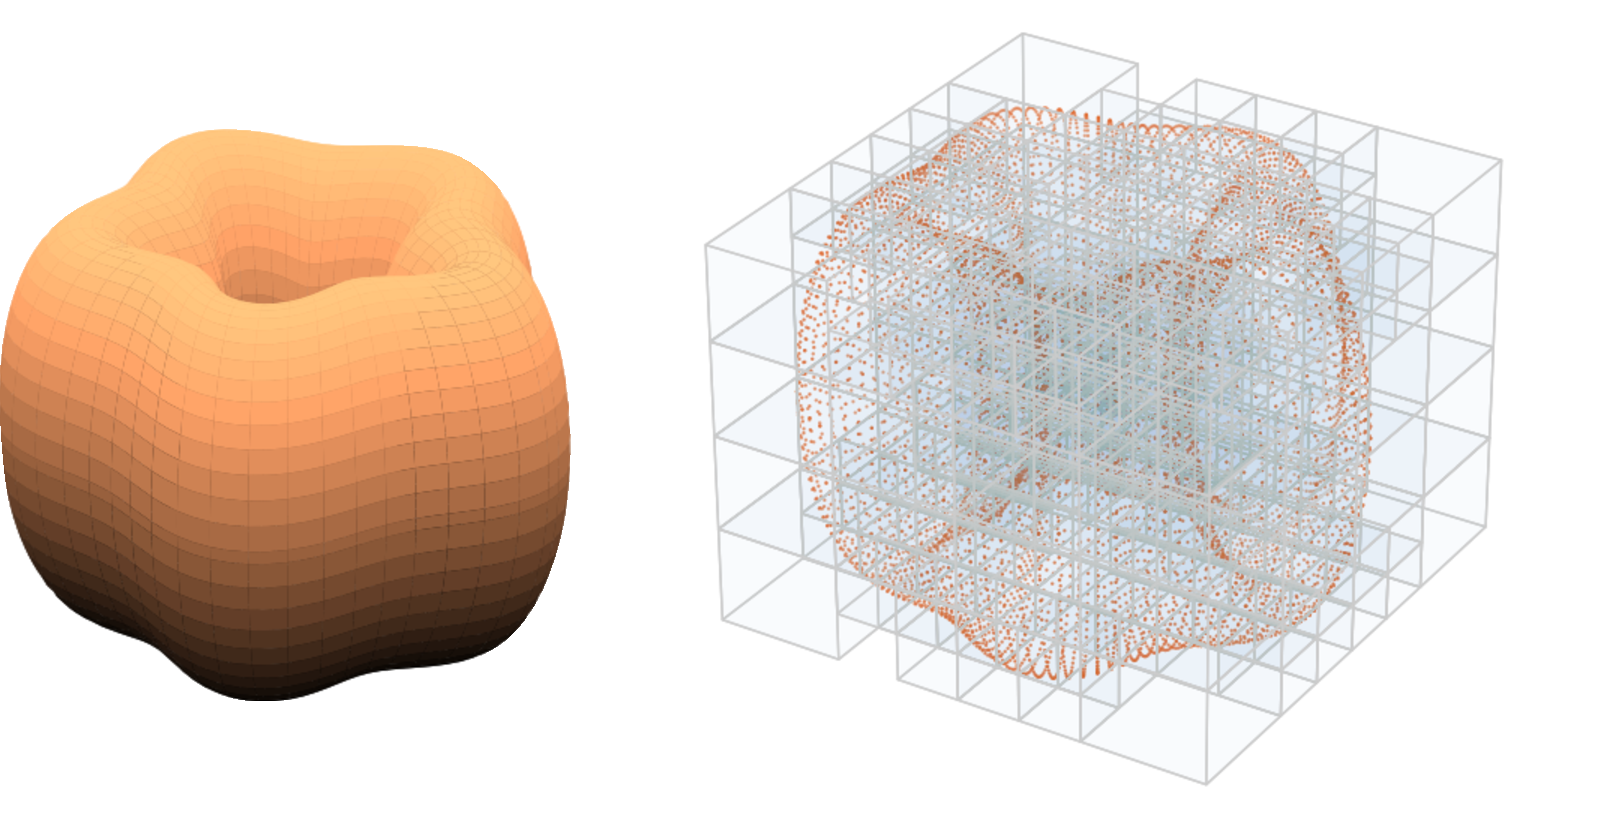
\includegraphics[width=0.7\textwidth]{ch_1/octree_example.pdf}
    \caption{An adaptive octree for random point data placed on the surface of a `wiggly torus' test geometry. The user defines the level of recursion via a threshold for the maximum number of particles in a given node.}
    \label{fig:octree_example:sec_1_2}
\end{figure}

In addition to the $\mathsf{T}^{P2M}$, $\mathsf{T}^{M2L}$ and $\mathsf{T}^{L2P}$ the FMM also require operators that can translate the expansion centre of a multipole or local expansion, $\mathsf{T}^{L2L}$, $\mathsf{T}^{M2M}$, an operator that can form a local expansion from a set of points $\mathsf{T}^{P2L}$, and apply a multipole approximation to a set of points, $\mathsf{T}^{M2P}$, finally we need define a $P2P$ operator as short hand for direct kernel evaluations. Algorithm (1) provides a brief sketch of the full FMM algorithm.

\begin{algorithm}
\caption{\textbf{Adaptive Fast Multipole Method}: \gls{FMM} literature distinguishes between types of relationships  between neighbouring nodes with the concept of \textit{interaction lists}. There are four such lists for a given node $B$, called $V$, $U$, $W$ and $X$. For a leaf node $B$, the $U$ list contains $B$ itself and leaf nodes adjacent to $B$. and the $W$ list consists of the descendants of $B$'s neighbours whose parents are adjacent to $B$. For non-leaf nodes, the $V$ list is the set of children of the neighbours of the parent of $B$ which are not adjacent to $B$, and the $X$ list consists of all nodes $A$ such that $B$ is in their $W$ lists. The non-adaptive algorithm is similar, however the $W$ and $X$ lists are empty.}
\label{alg:fmm:sec_1_2}
\begin{algorithmic}

    \State $N$ is the total number of points
    \State $s$ is the maximum number of points in a leaf node.

    \State
    \State \textbf{Step 1: Tree construction}
    
    \For{each node $B$ in \textit{preorder} traversal of tree}
        \State subdivide $B$ if it contains more than $s$ points.
    \EndFor
    \For{each node $B$ in \textit{preorder} traversal of tree}
        \State construct \textit{interaction lists}, $U$, $V$, $X$, $W$
    \EndFor
    
    \State 
    \State \textbf{Step 2: Upward Pass}
    \For{each leaf node $B$ in \textit{postorder} traversal of the tree}
    \State \textbf{P2M}: compute multipole expansion for the particles they contain.
    \EndFor
    \For{each non leaf node $B$ in \textit{postorder} traversal of the tree}
    \State \textbf{M2M}: form a multipole expansion by translating the expansion centre of its children to its centre and summing their multipole expansion coefficients.
    \EndFor

    \State
    \State \textbf{Step 3: Downward Pass}
    \For{each non-root node $B$ in \textit{preorder} traversal of the tree}
    \State \textbf{M2L}: translate multipole expansions of nodes in $B$'s $V$ list to a local expansion at $B$.
    \State \textbf{P2L}: translate the charges of particles in $B$'s $X$ to the local expansion at $B$.
    \State \textbf{L2L}: translate $B$'s local expansion to its children by translating its expansion centre to the centre of its children, and assigning the same coefficients.
    \EndFor 

    \For{each leaf node $B$ in \textit{preorder} traversal of the tree}
    \State \textbf{P2P}: directly compute the local interactions using the kernel between the particles in $B$ and its $U$ list.
    \State \textbf{L2P}: translate local expansions for nodes in $B$'s $W$ list to the particles in $B$.
    \State \textbf{M2P}: translate the multipole expansions for nodes in $B$'s $W$ list to the particles in $B$.
    \EndFor
\end{algorithmic}
\end{algorithm}

\begin{figure}
    \centering
    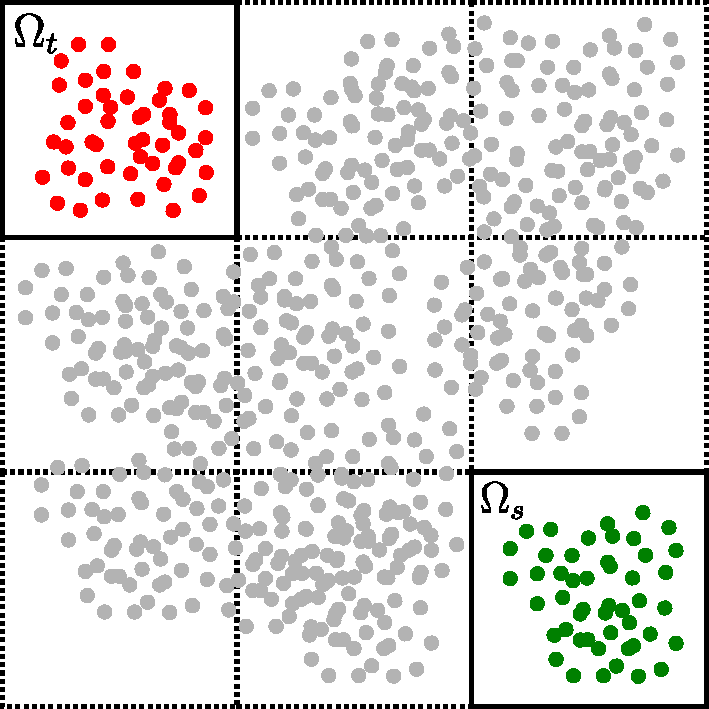
\includegraphics[width=0.5\textwidth]{ch_1/single_level_r2.pdf}
    \caption{Two well separated clusters $\Omega_t$ and $\Omega_s$ where we can apply a low-rank approximation.}
    \label{fig:single_level_r2:sec_1_2}
\end{figure}

In its original analytical form the applicability of the FMM is limited by the requirement for an explicit multipole and local expansions, as well as a restriction to matrix vector products. This lead to the development of algebraic variants that operate on the matrix represented by (\ref{eq:potential_matvec:sec_1_2}) directly, without the need for geometrical considerations via an octree. Examples include, the $\mathcal{H}$ matrix \cite{hackbusch1999sparse}, $\mathcal{H}^2$ matrix \cite{borm2003short}, hierarchically semi-separable (HSS) \cite{chandrasekaran2007fast}, and hierarchically off-diagonal low-rank (HODLR) \cite{ambikasaran2013mathcal} matrices.

These methods all represent the system matrix in (\ref{eq:potential_matvec:sec_1_2}) using a stored hierarchical matrix factorisation. Once this factorisation is computed, it can be used again - allowing for simple extensions to matrix-matrix products. Furthermore, an explicit matrix forms also allows for optimal matrix inversion algorithms.

Consider an index set $I$, corresponding to the indices of all points $\{ x_i \}_{i=1}^N$ in a given discretisation. The general approach of these methods is to partition $I$ in such a way that we can exploit the low-rank interactions between distantly separated clusters of particles. Initially, an $n$-ary `cluster tree' $\mathcal{T}_I$, with a set of nodes $T_I$, is formed such that

\begin{enumerate}
    \item $T_I \subseteq \mathcal{P}(I) \setminus \{ \emptyset \}$, meaning each node  of $\mathcal{T}_I$ is a subset of the index set $I$, here $\mathcal{P}(I)$ denotes the power set of $I$.
    \item $I$ is the root of $\mathcal{T}_I$
    \item The number of indices in a leaf node $\tau \in T_I$ is such that $|\tau| \leq C_{\text{leaf}}$ where $C_{\text{leaf}}$ is a small constant.
    \item Non leaf nodes $\tau$ have $n$ child nodes $\{ \tau \}_i^n$, and is formed of their disjoint union $\tau = \cupdot_{i=1}^n \tau_i$ 
\end{enumerate}

Cluster trees may in general be $n$-ary, however common implementations are as binary trees. Using a cluster tree, one forms a `block tree', $\mathcal{T}_{I \times I}$. Each node, or `block', of a block tree, $N(\tau \times \sigma)$, corresponds to the clusters represented by indices $\tau \subseteq I$ and $\sigma \subseteq I$ respectively. The $\mathcal{H}$ and $\mathcal{H}^2$ representations are `strongly admissible', meaning that well separated blocks as in figure (\ref{fig:low_rank:sec_1_1}) can be compressed. In contrast, the HSS and HODLR approaches are `weakly admissible', and also consider adjacent clusters to be compressible. Admissibility is calculated by forming a bounding box around clusters, and checking their separation along each dimension \cite{borm2003introduction}. Furthermore, as in the \gls{FMM} which creates parent multipole expansions for a given node from that of its children, and vice versa for local expansions, an analagous approach is taken by $\mathcal{H}^2$ and HSS matrices, referred to as `nested bases'. These different approaches are succinctly visualised in figure (\ref{fig:ambikasaran_hierarchical:sec_1_2}). 

Expressed in this way the matrix implicit in the FMM (alg. (\ref{alg:fmm:sec_1_2})), can be seen to be a member of the $\mathcal{H}^2$ class of matrices. Therefore the algorithms developed for algebraic approaches for matrix vector products similarly recover optimal $O(N)$ scaling in the best case, with the additional benefit of easy extension to matrix matrix products, and matrix inversion in optimal complexity \cite{borm2003introduction}.

\begin{figure}
    \centering
    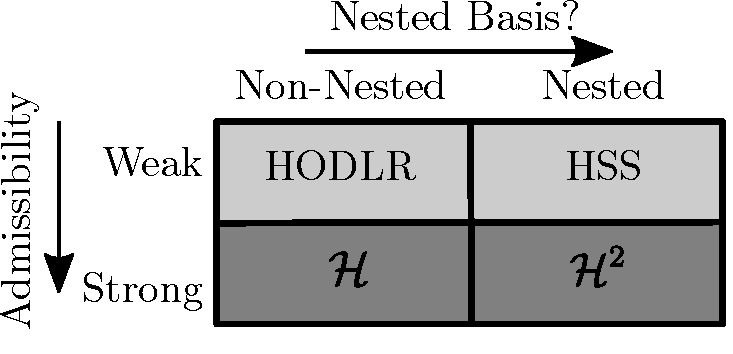
\includegraphics[width=0.5\textwidth]{ch_1/ambikasaran_hierarchical.pdf}
    \caption{Matrix containing common algebraic alternatives to the FMM, adapted from \cite{ambikasaran2013fast}.}
    \label{fig:ambikasaran_hierarchical:sec_1_2}
\end{figure}

From a computational perspective, the trade-off between these analytical and algebraic approaches for the FMM are best expressed in terms of the ratio of compute (\gls{flops}) to memory (bytes), or `arithmetic intensity'. The analytical \gls{FMM} has a high arithmetic intensity, due to its matrix free nature. However, using explicit $\mathcal{H}^2$ representations requires one to compute and store the full hierarchical matrix in memory, resulting in increased memory movement costs, both vertically on a single node, and horizontally in a distributed memory setting. 

A third `semi-analytical' method, combining the best of the purely analytical and algebraic methods are known as `black box', or `kernel independent', \gls{FMM}s \cite{Ying:2004:JCP,fong2009black,martinsson2007accelerated}. These methods mimic the algorithmic structure of the analytical FMM, with its matrix free nature, however the low rank representations they construct are done so independently of the kernel, hence the name `black box'. We contrast two common black box methods in figure (\ref{box:kifmm_vs_bbfmm:sec_1_2}), the underlying difference being in their representation of translation operators.

Black box methods are preferable from a software standpoint for three reasons: (1) generic interfaces can be built for a variety of kernels, (2) they have reduced storage requirements in comparison to purely algebraic approaches, and (3) the majority of computations are simple matrix vector products that are readily expressed with BLAS L2 operations. 

Few studies have directly compared the efficacy of analytical, semi-analytical and algebraic FMM variants. Yokota et. al. compare the matrix vector products of (\ref{eq:n_body:sec:1_1}) performed by the \gls{FMM} using the ExaFMM package \cite{exafmm} and HSS factorisations using the STRUMPACK package \cite{rouet2016distributed}. Thet


Yokota et. al \cite{yokota2015fast}, find similar single node performance between ...

. However the trend in computing architectures is towards systems with relatively cheap computations and significantly more expensive memory movements \cite{dongarra2017extreme}. This is especially the case in large scale distributed systems, where memory movements between nodes dominate compute times. More on the architectures of exascale systems here ...

We prefer the kernel-independent FMM introduced by Ying et. al \cite{Ying:2004:JCP}. Here, we are able to represent translations as in figure [YING FIGURE]. Here translations can be readily accelerated with randomized techniques for matrix compression \cite{halko2011finding}. Consider the $T^{M2L}$ operator, this dominates the cost of an FMM as its interaction list, $V$,  for a given non-leaf node is $|V| = 189$ in $\mathbb{R}^3$ and $|V|=27$ in $\mathbb{R}^2$.

... Digression on the acceleration of the M2L operator using randomized svd

Numerous techniques have emerged to accelerate the calculation of $T^{M2L}$ in a black box setting. By focussing on the rotational symettry of interactions (see figure [M2L SYMETTRY FIGURE), and their translational invariance, we can avoid redundant calculations, while pre-computing and storing the remainder.

We conclude by mentioning that the \gls{FMM} and its variants are not the only technique available to accelerate (\ref{eq:n_body:sec:1_1}), for problems in which only uniform resolution is required the \gls{FFT}, which has corresponding distributed memory implementations [FAST FFT REFERENCE SOFTWARE]. However, we are commonly interested in multiscale problems in which neighbouring nodes can be of differing sizes, in which case multigrid approaches have shown similar efficacy to the FMM \cite{gholami2016fft}, however has an unfavourable communication cost (see appendix [FFT COMMUNICATION COST]). However, a multigrid approach does not allow for a re-use of FMM data structures (sec. \ref{sec:3_2}) for other fast algorithms we are interested in implementing, and aim to present as a unified framework with maximum code re-use.

\newpage
\begin{multicols}{2}
    % \begin{figure}
    \begin{tcolorbox}[width=1\linewidth, halign=left, colframe=black, colback=gray!10, boxsep=2mm, arc=0mm, left=1pt,right=1pt,top=0pt,bottom=0pt]
    \textbf{Kernel-Independent FMM (KIFMM)}
        
    The KIFMM approximates the multipole expansion for a given leaf node containing particles $\{ y_j \}_j^N$ with charges $\{ q_j\}_j^N$ by evaluating their potential directly (\ref{eq:potential_matvec:sec_1_2}) at corresponding evenly spaced points on a `check surface', displayed in blue.

    \vspace{2pt} 
    \begin{center}
        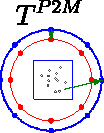
\includegraphics[height=2.1cm]{ch_1/kifmm2.pdf}
    \end{center} 
    \vspace{2pt} 

    This is matched to $N_e$ `equivalent charges', $\mathsf{q}^e$, placed evenly on a the (red) equivalent surface at $\{ x_i \}_i^{N_e}$. These surfaces are taken to be circles in $\mathbb{R}^2$ and cubes in $\mathbb{R}^3$. They perform a Tikhonov-regularised least squares fit to calculate  $\mathsf{q}^e$, which plays the role of the \textit{multipole expansion}.
    
    \begin{flalign*}
        \mathsf{q}^e = (\alpha I + \mathsf{K}^* \mathsf{K})^{-1}\mathsf{K}\mathsf{q}^{\text{node}}
    \end{flalign*}

    where $\mathsf{q}^{\text{node}}$ are the charges in the leaf node. Using a similar framework, involving equivalent and check surfaces, the $T^{M2M}$, $T^{M2L}$, $T^{L2L}$ and $T^{L2P}$ operators are also calculated with Tikhonov-regularised least squares fitting, and are sketched below.

    \vspace{2pt} 
    \begin{center}
        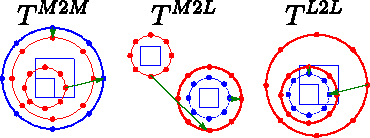
\includegraphics[height=2.1cm]{ch_1/kifmm.pdf}
    \end{center} 
    \vspace{2pt} 

    The KIFMM is designed for non-oscillatory kernels, such as the Laplace kernel of our didactic example, though in practice works well with low-frequency oscillatory problems, with extensions to high frequency problems \cite{engquist2007fast}.
    
    The least-squares fit can be pre-computed for each given geometry, and re-used. Additionally, as the KIFMM decomposes into a series of matrix vector products, it is well suited to software implementations.
    \end{tcolorbox} 
        
    \columnbreak
    \begin{tcolorbox}[width=1\linewidth, halign=left, colframe=black, colback=gray!10, boxsep=2mm, arc=0mm, left=1pt,right=1pt,top=0pt,bottom=0pt]
    \textbf{Black-Box FMM (bbFMM)}
    
    \setlength{\belowdisplayskip}{0pt} \setlength{\belowdisplayshortskip}{0pt}
    
    \setlength{\abovedisplayskip}{0pt} \setlength{\abovedisplayshortskip}{0pt}


    An $n$ point interpolation scheme for the kernel is constructed sequentially over each variable, 

    \begin{flalign*}
        &K(x, y) \approx \sum_{l=1}^n K(x_l, y)w_l(x) \\
        &K(x, y) \approx \sum_{l=1}^n\sum_{m=1}^nK(x_l, x_y)w_l(x)w_m(x)
    \end{flalign*}

    with coefficients $w_l(x)$ and $w_m(x)$. The bbFMM uses first kind Chebyshev polynomials, $T_n$ to interpolate the kernel, defined as,

    \begin{flalign*}
        T_n(x) = \cos(n \theta), \> \> \text{where } x = \cos(\theta)
    \end{flalign*}

    over the closed interval $x \in [-1, 1]$. The roots, $\{ \bar{x}_m \}$ , known as Chebyshev nodes are defined as,

    \begin{flalign*}
        \bar{x}_m = \cos(\theta_m) = \cos(\frac{(2m-1\pi)}{2n}) \\
    \end{flalign*}
    
    This is a well known, stable, uniformly convergent, interpolation scheme, that doesn't suffer from Runge's phenomenon \cite{fong2009black}. An $n$ point Chebyshev approximation to a given function, $g(x)$ with $p_{n-1(x)}$, can be written as,

    \begin{flalign*}
        &p_{n-1}(x) = \sum_{k=1}^{n-1}c_k T_k(x) \\
        \text{where, } &c_k = \begin{cases}
            \frac{2}{n} \sum_{l=1}^ng(\bar{x}_l)T_k(\bar{x}_l), \text{ if } k > 0\\
            \frac{1}{n} \sum_{l=1}^ng(\bar{x}_l), \text{ if } k = 0
        \end{cases}
    \end{flalign*}

    we recognise,

    \begin{flalign*}
        &p_{n-1}(x) = \sum_{l=1}^ng(\bar{x}_l)S_n(\bar{x}_l, x) \\
        \text{with, } &S_n(x, y) = \frac{1}{n} + \frac{2}{n}\sum_{k=1}^{n-1}T_k(x)T_k(y)
    \end{flalign*}

    When applied to our generic interpolation for the kernel,

    \begin{flalign*}
        K(x, y) &\approx\\
        &\sum_{l=1}^n\sum_{m=1}^n K(\bar{x}_l, \bar{y}_m) S_n(\bar{x}_l, x) S_n(\bar{y_m}, y)
    \end{flalign*}

    which can be substituted into (\ref{eq:two_box_calc:sec_1_2}), recovering linear complexity as long as the number of Chebyshev nodes is small, $n \ll N$.

    % Returning to the low-rank decomposition of the kernel (\ref{eq:low_rank_decomposition_of_kernel:sec_1_2}),
    
    % \begin{flalign*}
    %     K(x,y) \approx \sum_{p=0}^{P-1}B_p(x)C_p(y)
    % \end{flalign*}
    \end{tcolorbox}

\end{multicols}
\noindent\begin{minipage}{\textwidth}
    \captionof{figure}{The formulations of the kernel-independent FMM methods, the KIFMM \cite{Ying:2004:JCP} and the bbFMM \cite{fong2009black}.}
    \label{box:kifmm_vs_bbfmm:sec_1_2} 
\end{minipage}

    
% - FMM vs other methods (FFT, Multigrid)
% - Uniform resolution use FFT, introduce FFT as first 'fast algorithm', however has unfavourable communication cost.
% - For non-uniform global problems also have multigrid methods as an alternative, also O(N) cost for elliptic/hyperbolic PDE problems. Gholami, Malhotra, Sundar, Biros (2016) - multigrid decent.

% - Fast translation operators crucial - take up a lot of time of the FMM, whatever its implementation.
%     - analytical options for fast translation operators.
%         - Rotation of spherical harmonics 92
%         - Block FFT 36
%         - Planewaves 50

%     - Accelerating M2L step
%         - level-skip M2L method 91
%         - 8,4,2 box method 93
%         - methods that use dual tree traversal alongside multipole acceptance criterion to construct optimal interaction lists 34

%     - Variable expansion order
%         - VFMM 85
%         - Guassian VFMM 20
%         - optimal parameter FMM 28
%     - intuition = boxes further away can afford to be of lower expansion order without loss of accuracy.

%     - Can store translations as matrices - typical optimisation
%         - matrix compression techniques - randomized techniques too.
%         - matrix techniques allow one to take advantage of BLAS
%             - maximises cache utilisation 39 (And US in PyExaFMM)
%         - Combination of techniques like Chebychev with SVD 38
%             - essentially systematic way of doing something like variable expansion order.

% - FMM is a method that has the analytical form to generate small (low-rank) off-diagonal matrices without needing to rely on a numerical approximation method.

% - making better use of translational invariance and rotational symmetry of the interacti